\documentclass{beamer}
\usepackage[french]{babel}
\usepackage{beamerthemesplit} % new 
\usepackage[utf8]{inputenc}
\usepackage{tabularx} % in the preamble
\usepackage{listings}
\usetheme{Warsaw}
\begin{document}
\lstset{
	tabsize=4,
	language=Java,
        basicstyle=\scriptsize,
        columns=fixed,
        extendedchars=true,
        breaklines=true,
		frame=single,
        showtabs=false,
        showspaces=false,
        showstringspaces=false,
        identifierstyle=\ttfamily,
        keywordstyle=\color[rgb]{0,0,1},
        commentstyle=\color[rgb]{0.133,0.545,0.133},
        stringstyle=\color[rgb]{0.627,0.126,0.941},
        numbers=left, 
        numberstyle=\tiny,
        xleftmargin=\parindent
}

\title{Technologies mobiles} 
\author{Olivier Levitt} 
\date{\today} 
\AtBeginSubsection[]
{
  \begin{frame}
  \frametitle{Sommaire}
  \tiny{\tableofcontents[currentsubsection]}
  \end{frame}
}


\frame{
\titlepage
\begin{center}

\includegraphics[width=60pt]{google-android.jpg}

\includegraphics[width=60pt]{ios.png}

\includegraphics[width=60pt]{wp8.jpg}

\includegraphics[width=60pt]{bb10.jpg}
\end{center}
} 

\frame{\frametitle{Sommaire}\tableofcontents} 
 
\section{Présentation et objectifs du cours}
\subsection{Organisation administrative}
\frame{
\frametitle{Planning}
\begin{itemize}
  \item{30 janvier : 3h de cours, 3h de TP}
  \item{6 février : 3h de cours}
  \item{13 février : 6h de TP}
  \item{Validation des sujets de projet avant le 20 février}
  \item{20 février : 6h de TP dédiées au projet}
  \item {? mars : Soutenance du projet}
\end{itemize}
}

\frame{
\frametitle{Evaluation}
\begin{itemize}
  \item{Projet : création d'une application}
  \item{Groupe de 2}
  \item{Sujet ``libre''}
  \item{6h de TP dédiées au projet + \textbf{travail personnel}}
  \item{Soutenance / Présentation de l'application}
\end{itemize}
}
\frame{
\frametitle{Evaluation, exemples de sujets}
\begin{itemize}
  \item{PamplemousseViewer v2}
  \item{Gestion d'une bibliothèque}
  \item{Quiz}
  \item{Tape-taupes}
  \item{Serveur SMS}
  \item{Achievements}
\end{itemize}
}
\subsection{Contexte et objectifs}
\frame{
\frametitle{Contexte et objectifs}
\begin{itemize}
  \item Smartphones, tablettes et assimilés (TV, montre, autoradio, consoles de
  jeu \ldots)
  \item Développement d'application, pas de dev de la plateforme
  \item 1ère partie : le développement mobile en général
  \item 2ème partie : application sous android
\end{itemize}
}

\section{Le développement mobile} 
\subsection{Spécificités du développement mobile}
\frame{
\frametitle{Des appareils suréquipés}
\begin{itemize}
  \item Téléphonie (SMS, MMS, appels)
  \item Internet (GPRS, EDGE, 3G, 4G, WIFI)
  \item Réseaux locaux (Bluetooth, réseaux adhoc, NFC)
  \item Capteurs (Luminosité, proximité)
  \item Localisation (GPS, triangulation, SSID wifi)
  \item Notifications (Vibreur, haut-parleurs, LED)
  \item Photo / vidéo
  \item Stockage de données (Mémoire flash, SD externe, SQLite)
  \item Interactions (Ecran tactile, gestures, boutons physique)
  \item Et encore d'autres \ldots
\end{itemize}
Et des API pour utiliser tout ça !
}
\frame{
\frametitle{Des contraintes techniques importantes}
\begin{itemize}
  \item Processeur
  \item Mémoire RAM
  \item Stockage de données
  \item Gestion de la batterie
  \item Stabilité et débit de la connexion internet
  \item Cycle de vie de l'application
  \item Taille d'écran 
  \item Inputs atypiques (clavier virtuel, gestures, peu de boutons \ldots)
\end{itemize}
Contraintes à garder en tête en permanence.
}
\frame{
\frametitle{La fragmentation}
Une application publiée sur le google playstore cible plus de 2400 appareils
différents !\\
\begin{itemize}
   \item ``Write once, run everywhere'' ?
   \item Comment tester / débugger pour tous ces appareils ?
  \item Eviter de géner l'utilisateur (versions HD, appareils non compatibles)
  \item S'adapter quand une fonctionnalité n'est pas disponible
\end{itemize}
}
\frame{
\frametitle{La fragmentation, taille d'écran}
Comment gérer toutes les tailles d'écran ? 
\begin{itemize}
  \item Montres connectées : de 1 à 2 pouces
  \item Smartphones lowcost : 3 pouces (Galaxy pocket, galaxy Y)
  \item Smartphones high-end : 4 à 5 pouces (IPhone 5, HTC 8X, nexus 4)
  \item Phablets : 5 à 6 pouces (Galaxy note, HTC butterfly)
  \item Tablettes : 7 pouces (Nexus 7, IPad mini), 8 pouces (Archos 80g9), 10 pouces (Nexus 10, IPad)
\end{itemize}
}


\frame{
\frametitle{De nombreuses autres sources de fragmentation}
\begin{itemize}
  \item Versions de l'OS
  \item Résolutions d'écran
  \item Elements hardware présents
  \item Puissance
  \item Modifications constructeur / ``rom custom''
  \item \ldots
\end{itemize}
}
\frame{
\frametitle{Des Ecosystèmes forts}
\begin{itemize}
  \item Obligation d'utiliser le SDK fourni
  \item Suivre les guidelines
  \item Restrictions liées à la plateforme
  \item Utilisation des services de la plateforme
  \item Processus de déploiement des applications
  \item Règles des ``store'' (validation, monétisation \ldots)
\end{itemize}
}
\subsection{Présentation des différents OS mobile}
\frame{
\frametitle{iOS}

\includegraphics[width=60pt]{ios.png}
\begin{itemize}
  \item Soutenu par Apple
  \item Présenté le 9 janvier 2007
  \item Dédié aux produits apple (iPhone, iPad, iPod)
  \item 400 millions d'appareils (Septembre 2012)
  \item Programmation en objective-C, sur mac OS X uniquement
  \item Appstore : validation + 100\$ / an
\end{itemize}
}
\frame{
\frametitle{Android}


\includegraphics[width=60pt]{google-android.jpg}
\begin{itemize}
  \item Soutenu par Google
  \item 1.0 en septembre 2008, 1.5 en avril 2009
  \item Plus de 2400 appareils officiellement supportés, plus de 50 constructeurs
  \item 480 millions d'appareils activés (Septembre 2012)
  \item Programmation en JAVA, sur windows / OS X / linux
  \item Open-source
  \item Google playstore : pas de validation + 25\$
\end{itemize}
}
\frame{
\frametitle{Windows phone 8}


\includegraphics[width=60pt]{wp8.jpg}
\begin{itemize}
  \item Soutenu par Microsoft
  \item Présentation au public le 29 octobre 2012
  \item Successeur de windows phone 7 (logique)
  \item Plusieurs constructeurs dont Nokia, HTC et Samsung
  \item Programmation en C\# sur windows 
  \item Windows marketplace : validation + 100\$ / an
\end{itemize}
}
\frame{
\frametitle{Blackberry 10}


\includegraphics[width=60pt]{bb10.jpg}
\begin{itemize}
  \item Soutenu par RIM (Research in motion)
  \item Présentation au public le 30 janvier 2012 (!)
  \item Appareils produits par RIM
  \item C / C++, HTML5, Adobe AIR, Portage android
  \item Blackberry appworld : validation + gratuit
\end{itemize}
}
\frame{
\frametitle{Ubuntu for phones}
\begin{itemize}
  \item Soutenu par Canonical
  \item Teaser le 2 janvier 2012, testable sur galaxy nexus fin février
  \item Premiers ubuntu phones promis pour début 2014
  \item Facilement utilisable sur les téléphones android ?
  \item HTML5, C/C++ + QML
  \item Open-source
  \item Peu d'infos sur le store
\end{itemize}
}
\frame{
\frametitle{Firefox OS}
\begin{itemize}
  \item Soutenu par Mozilla
  \item Premiers téléphones présentés le 22 janvier (geeksphone), disponibles en
  février ?
  \item Simulateur sous forme d'addon firefox
  \item HTML5
  \item Open-source
  \item Peu d'infos sur le store
\end{itemize}
}
\section{Le développement sur android} 

\subsection{Mise en place}
\frame{
\frametitle{Les marque-pages}
\begin{itemize}
  \item www.frandroid.com (actu FR)
  \item www.androidpolice.com (actu EN)
  \item www.androidcentral.com (actu EN)
  \item www.d.android.com (la bible EN)
  \item www.stackoverflow (Q/A EN)
  \item \#android et \#android-dev sur freenode (chat irc EN)
  \item www.breizhjug.org et www.paug.fr (communautés FR)
  \item www.google.fr (réservoir à tutoriels)
\end{itemize}
}
\frame{
\frametitle{Avant de commencer, la checklist}
Obligatoire :\\
\begin{itemize}
  \item Des (bonnes) bases de programmation en JAVA
  \item Un ordinateur (Windows, Linux, Mac OS X)
\end{itemize}
Conseillé :\\
\begin{itemize}
  \item Un appareil android (l'émulateur est \ldots moyen)
  \item Parler anglais
  \item Suivre l'actualité
\end{itemize}
}
\frame{
\frametitle{Les niveaux d'API}
\begin{table}
\begin{tabular}{|l|c|c|c|r|}
  \hline
  Version & Nom & API level & Distribution & Cumulé \\
  \hline
  1.5 & Cupcake & 3 & 0\% & 0\% \\
  1.6 & Donut & 4 & 0.2\% & 0.2\% \\
  2.1 & Eclair & 7 & 2.4\% & 2.6\% \\
  2.2 & Froyo & 8 & 9\% & 11.6\% \\
  2.3 & Gingerbread & 9/10 & 47.6\% & 59.2\% \\
  3.X & Honeycomb & 12/13 & 1.5\% & 60.7\% \\
  4.0.X & Ice cream sandwich & 15 & 29.1\% & 89.8\% \\
  4.1 & Jelly bean & 16 & 9\% & 98.8\% \\
  4.2 & Jelly bean & 17 & 1.2\% & 100\% \\
  \hline
\end{tabular}
\caption{\label{s}Répartition des versions pour les accès au google play sur la
dernière quinzaine de 2012}
\end{table}
}
\frame{
\frametitle{Présentation du SDK android}
Téléchargement gratuit : www.d.android.com/sdk
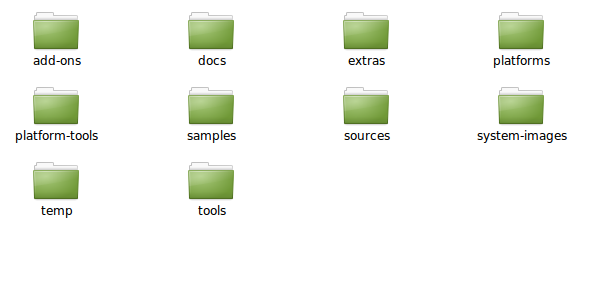
\includegraphics[width=300pt]{sdk.png}
}
\frame{
\frametitle{Présentation du SDK android}
\begin{itemize}
  \item add-ons : Google APIs
  \item docs : Copie de la documentation disponible sur d.android.com
  \item extras : Lib de compatibilité, lib pour les achats in-app \ldots
  \item platform-tools : Binaires de communication avec les appareils android
  (adb, fastboot \ldots)
  \item platforms : 1 dossier par niveau d'API téléchargé
  \item samples : Exemples de projets
  \item sources : Sources de chaque niveau d'API
  \item system-images : Images pour l'émulateur
  \item temp
  \item tools : Outils pour le dev (ddms, apkbuilder, lint \ldots)
\end{itemize}
}
\frame{
\frametitle{Plugin android pour eclipse : ADT}
Installation comme un plugin eclipse classique\\ 
\url{https://dl-ssl.google.com/android/eclipse/}\\
ADT fait le lien entre eclipse et le SDK android
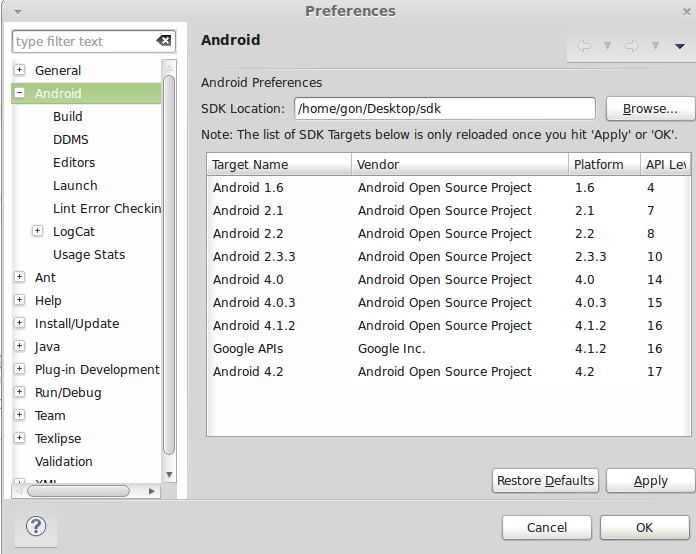
\includegraphics[width=100pt]{adt.png}
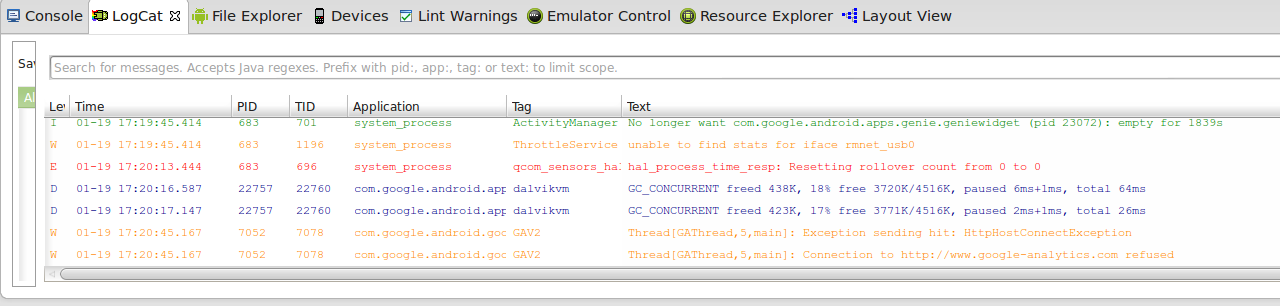
\includegraphics[width=200pt]{views.png}\\\\
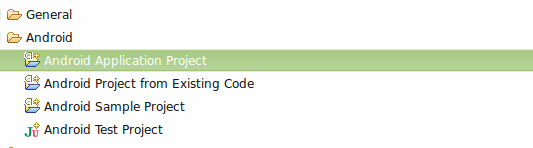
\includegraphics[width=100pt]{project.png}
}
\frame{
\frametitle{L'émulateur}
\begin{itemize}
  \item Utile pour tester certaines configurations
  \item ((très) très) lent
  \item Utiliser un appareil android à la place quand c'est possible
\end{itemize}
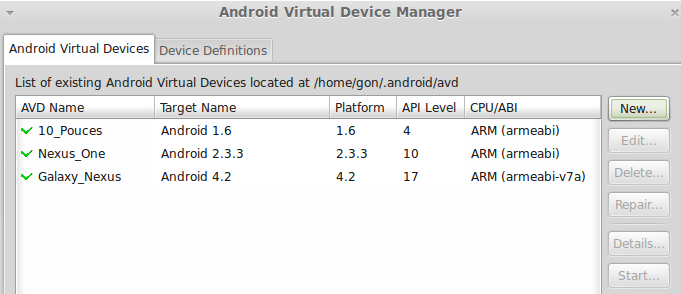
\includegraphics[width=300pt]{avd.png}
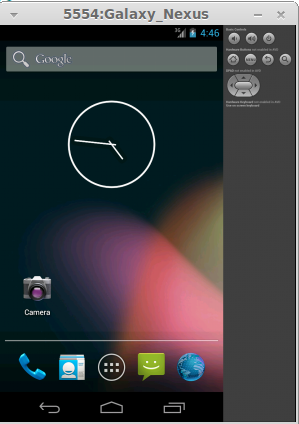
\includegraphics[width=42pt]{emu.png}
}
\frame{
\frametitle{Alternative à l'émulateur}
\begin{itemize}
  \item Problème : émuler de l'ARM sur nos machines x86
  \item Résultat : émulateur ((très) très) lent
  \item Solution proposée : porter android sur x86
  \item \url{http://www.android-x86.org/}
  \item \url{http://www.androvm.org/}
  \item 2012 : premiers appareils android sous x86 ``intel inside''
\end{itemize}
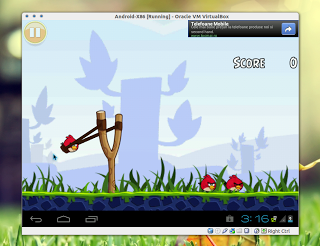
\includegraphics[width=170pt]{x86.png}
}
\subsection{Architecture}
\frame{
\frametitle{Organisation d'un projet android}
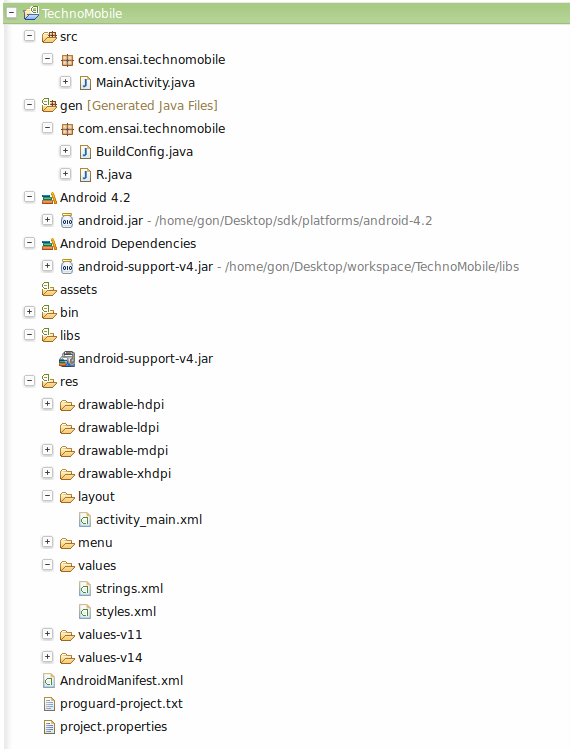
\includegraphics[width=150pt]{structure.png}
}
\frame{
\frametitle{Détail de l'organisation}
\begin{itemize}
  \item src : code source java
  \item gen : identifiants des ressources (généré par le sdk)
  \item Android 4.2 : jar correspondant à l'API cible
  \item Android Dependencies : jar rajoutés, correspond à libs
  \item assets : fichiers fournis avec l'app
  \item bin : résultat de la compilation (dont l'apk)
  \item libs : jar rajoutés
  \item res : ressources (layouts, strings, images \ldots)
  \item AndroidManifest.xml : métadonnées sur l'application, composants,
  permissions \ldots
  \item proguard-project.txt : configuration de proguard
  \item project.properties : généré par le sdk
 \end{itemize}
}
\frame{
\frametitle{AndroidManifest.xml : le coeur de l'application}
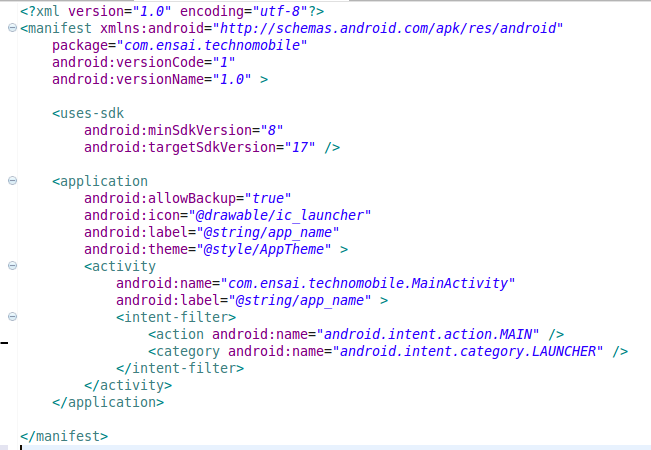
\includegraphics[width=150pt]{manifest.png}
\begin{itemize}
  \item Déclaration des composants
  \item Déclaration des permissions
  \item Déclaration d'autres métadonnées de l'application
  \item Analysé par l'OS à l'installation
 \end{itemize}
}
\begin{frame}[fragile]
\frametitle{Les permissions}
\begin{itemize}
  \item Obligatoires pour certaines fonctions (internet, géolocalisation,
  hardware \ldots)
  \item Les applications peuvent définir leurs propres permissions
  \item L'utilisateur est prévenu à l'installation / mise à jour
 \end{itemize}
 \begin{lstlisting}[language=XML]
<uses-permission android:name="android.permission.INTERNET"/>
<uses-permission android:name="android.permission.READ_SMS"/>
<uses-permission android:name="android.permission.CAMERA"/>
\end{lstlisting}
\end{frame} 


\frame{
\frametitle{Le système de ressources}
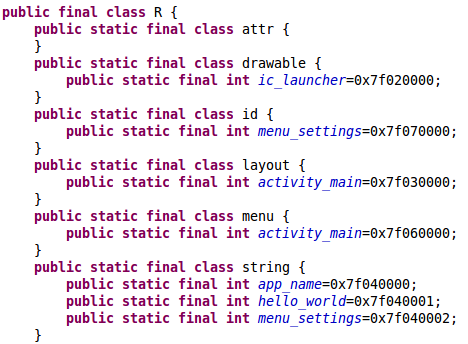
\includegraphics[width=150pt]{ressources.png}
\begin{itemize}
  \item Un identifiant est généré pour chaque ressource (drawable, layout, menu,
  values, style \ldots)
  \item Nom de l'identifiant = nom de la ressource sans l'extension
  \item Utiliser des ressources différentes en fonction de la configuration
  (values et values-fr, drawable et drawable-hdpi)
 \end{itemize}
}
\frame{
\frametitle{Déployer l'application}
\begin{itemize}
  \item Une application android = un APK (+/- équivalent d'un jar)
  \item Une application android doît être signée 
  \item Attention à ne pas perdre la clé !
  \item Création et signature de l'APK simple sous eclipse (export)
 \end{itemize}
}
\frame{
\frametitle{Processus de déploiement en dev}
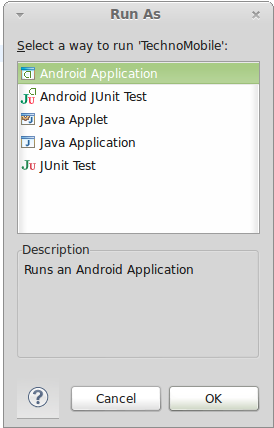
\includegraphics[width=50pt]{runas.png}
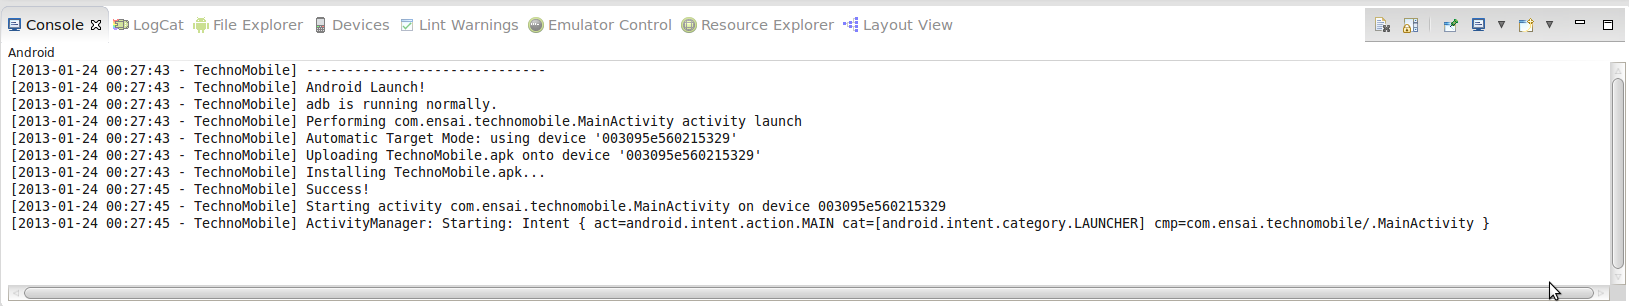
\includegraphics[width=300pt]{console.png}
\begin{itemize}
  \item Comme pour une application JAVA classique, ctrl + F11
  \item Eclipse demande au SDK de builder l'APK
  \item Eclipse signe l'APK avec la clé debug 
  \item Eclipse demande à adb (SDK) d'installer l'application
  \item Soit sur un appareil android connécté soit sur un émulateur
 \end{itemize}
}
\frame{
\frametitle{Distribuer l'application}
\begin{itemize}
  \item Distribution directe de l'APK (ex : pour tester, béta fermée)
  \item Publication sur le playstore, 25\$ à l'inscription
  \item Application gratuite ou payante (30\% pour google)
 \end{itemize}
}
\frame{
\frametitle{Déboguer l'application}
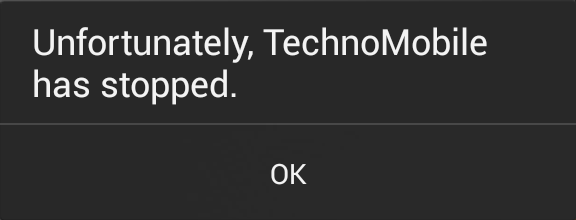
\includegraphics[width=120pt]{fc.png}
\begin{itemize}
  \item Si une exception n'est pas rattrapée, android tue l'application
  \item On parle de ``force close'' (FC)
  \item Comment déboguer une application qui tourne sur un appareil (ou
  émulateur) ?
 \end{itemize}
}
\frame{
\frametitle{Stacktrace of GTFO}
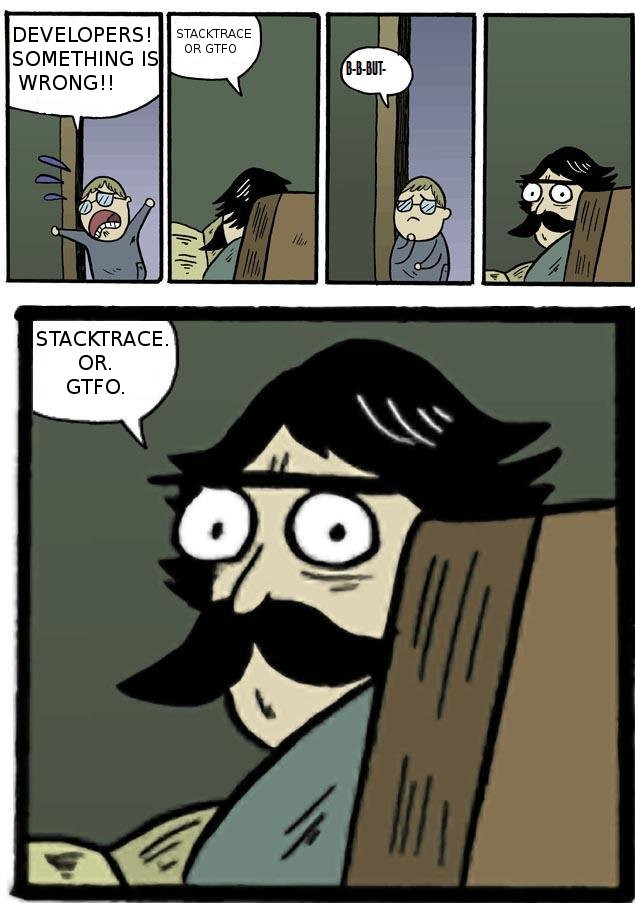
\includegraphics[width=120pt]{jacoj.jpg}
}
\frame{
\frametitle{Logcat, le sauveur}

\includegraphics[width=120pt]{logcat.jpg}
\begin{itemize}
  \item Le SDK fournit un outil très pratique : logcat
  \item On appelle logcat par adb : adb logcat ou on utilise la vue LogCat du
  plugin ADT
  \item Logcat affiche l'ensemble des logs, système et application
 \end{itemize}
}
\frame{
\frametitle{Logcat, exemple}
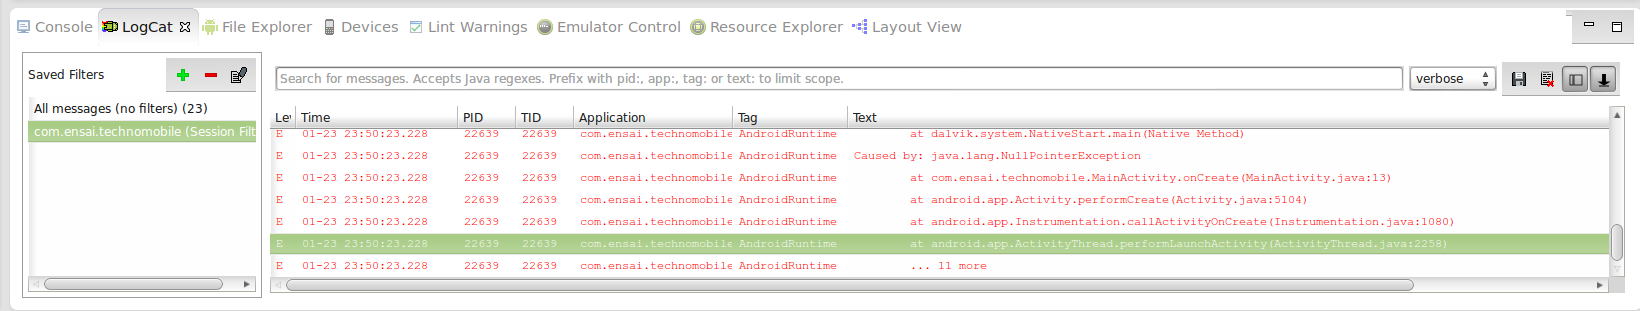
\includegraphics[width=340pt]{logeclipse.png}\\
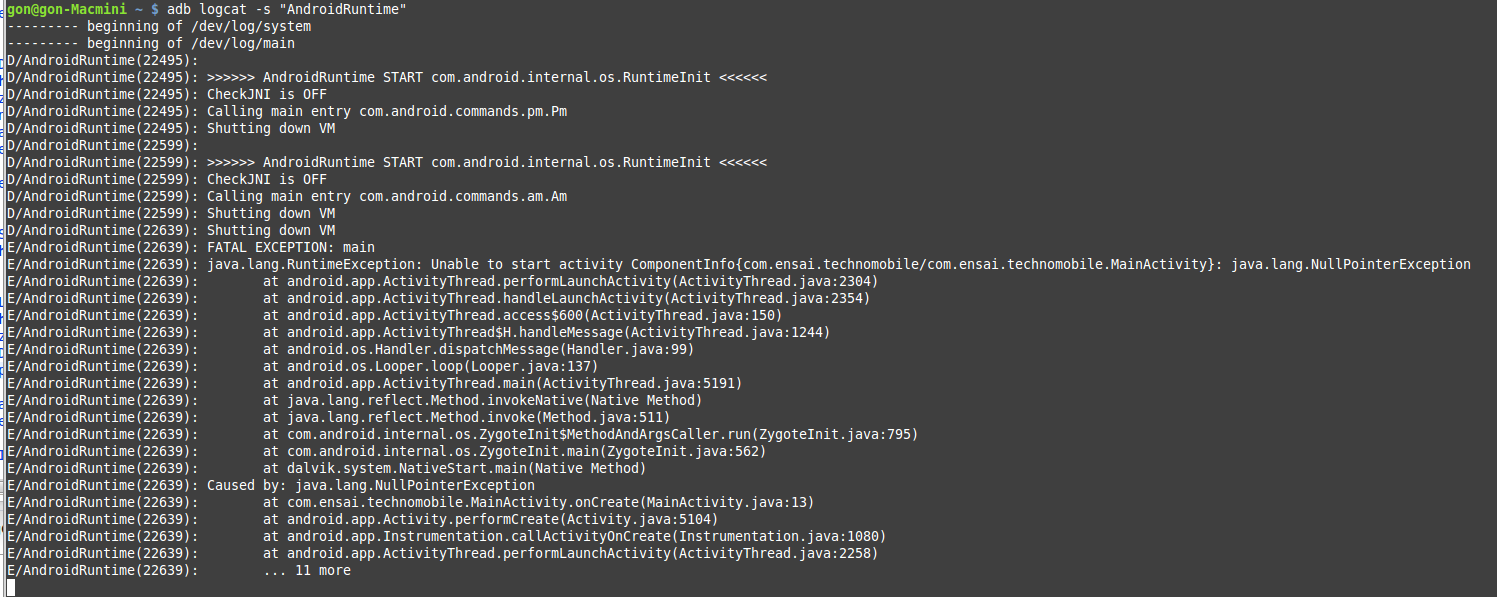
\includegraphics[width=340pt]{logterminal.png}
}
\begin{frame}[fragile]
\frametitle{Logcat, logging de l'application}
\begin{itemize}
  \item Oublier System.out.println() !
  \item 5 niveaux de gravité : ERROR, WARN, INFO, DEBUG, VERBOSE
  \item Possibilité dans adb logcat de filtrer par gravité et/ou TAG
  \item Pratique recommandée : un TAG par application
 \end{itemize}
 \begin{lstlisting}
public void sauvegarderScore(int score) {
        Log.i(TAG,"Sauvegarde du score "+score);
        if (score <= 0) {
            Log.w(TAG,"Le score est negatif");
        }
        try {
            //traitement
        }
        catch (Exception e) {
        	Log.e(TAG,"Erreur de score",e);
        }
}
\end{lstlisting}
\end{frame}
\subsection{IHM}
\frame{
\frametitle{Activity, le composant de base}
  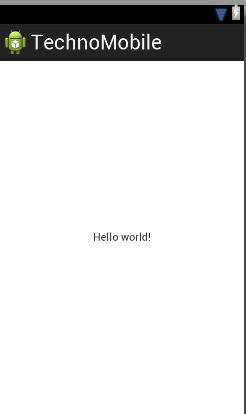
\includegraphics[width=50pt]{activity.png}
\begin{itemize}
  \item 1 activity {\raise.17ex\hbox{$\scriptstyle\sim$}}  un écran
  \item Une application peut avoir 0-n activities
  \item A ajouter dans le manifest
  \item Créer une classe java héritant de Activity 
 \end{itemize}
}

\frame{
\frametitle{Cycle de vie d'une activity} 
  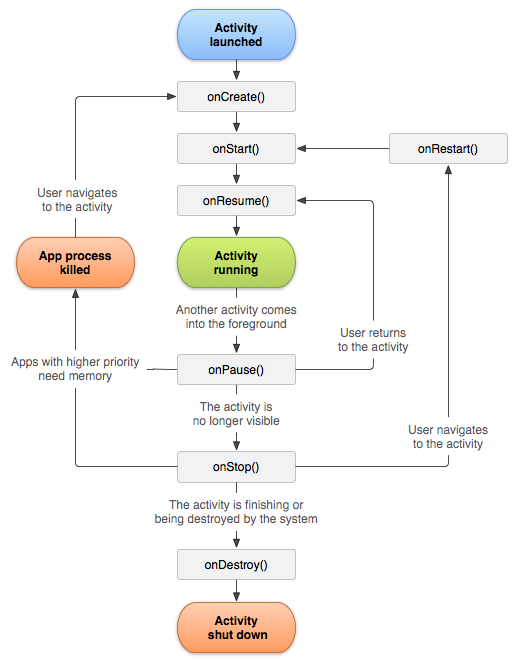
\includegraphics[width=150pt]{activity_lifecycle.png}
}
\begin{frame}[fragile]
\frametitle{Créer une activity : étendre Activity} 
\begin{lstlisting}
public Class MyActivity extends Activity {

    @Override
    protected void onCreate(Bundle savedInstanceState) {
        super.onCreate(savedInstanceState);
        setContentView(R.layout.activity_main);
    }
}
\end{lstlisting}
 \begin{itemize}
 \item onCreate est appellé à la création de l'activity (cf cycle de vie)
 \item appel obligatoire à super.onCreate
 \item le bundle savedInstanceState contient les informations en cas de
 relancement de l'activity
 \item savedInstanceState est null s'il s'agit du premier lancement
 \end{itemize}
\end{frame}
\begin{frame}[fragile]
\frametitle{L'organisation d'une activity : les layouts} 
\begin{lstlisting}
<LinearLayout 
	xmlns:android="http://schemas.android.com/apk/res/android"
    android:layout_width="match_parent"
    android:layout_height="match_parent">

    <TextView
        android:layout_width="wrap_content"
        android:layout_height="wrap_content"
        android:text="@string/hello_world" />

</LinearLayout>
\end{lstlisting}
 \begin{itemize}
 \item Ils sont définis en XML dans le dossier res/layout
 \item Ils définissent l'organisation des vues
 \item Eviter au maximum de modifier / créer les layouts au runtime
 \end{itemize}
\end{frame}
\begin{frame}[fragile]
\frametitle{Les Views}
   Une vue = un élement à l'écran
  \begin{itemize}
    \item TextView = Un texte
    \item EditText = Un champ de texte remplissable
    \item ImageView = Une image
    \item Button
    \item CheckBox
    \item Plein d'autres views de base dans android
    \item Possibilité de créer ses propres views en étendant View ou SurfaceView
 \end{itemize}
\end{frame}
\begin{frame}[fragile]
\frametitle{Les ViewGroups}
  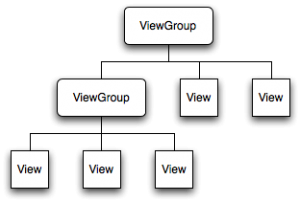
\includegraphics[width=150pt]{viewgroup.png}
  \begin{itemize}
 \item LinearLayout
 \item RelativeLayout
 \item ListView
 \item Plein d'autres
 \item Les vôtres :)
 \end{itemize}
\end{frame}
\begin{frame}[fragile]
\frametitle{Manipuler les éléments de l'UI en java}
Etape 1 : donner un identifiant à la vue
\begin{lstlisting}
<LinearLayout 
	xmlns:android="http://schemas.android.com/apk/res/android"
    android:layout_width="match_parent"
    android:layout_height="match_parent"
    android:id="@+id/monlayout">

    <Button
        android:layout_width="wrap_content"
        android:layout_height="wrap_content"
        android:id="@+id/monbouton"
        android:text="@string/hello_world" />

</LinearLayout>
\end{lstlisting}
\end{frame}
\begin{frame}[fragile]
\frametitle{Manipuler les éléments de l'UI en java}
Etape 2 : récupérer les réferences vers les views
\begin{lstlisting}
public Class MyActivity extends Activity {

    ViewGroup layout = null;
    Button bouton = null;

    @Override
    protected void onCreate(Bundle savedInstanceState) {
        super.onCreate(savedInstanceState);
        setContentView(R.layout.activity_main);
        layout = (ViewGroup) findViewById(R.id.monlayout);
        bouton = (Button) findViewById(R.id.monbouton);
    }
}
\end{lstlisting}
\end{frame}
\begin{frame}[fragile]
\frametitle{Manipuler les éléments de l'UI en java}
\begin{lstlisting}
public Class MyActivity extends Activity {

    ViewGroup layout = null;
    Button bouton = null;

    @Override
    protected void onCreate(Bundle savedInstanceState) {
        super.onCreate(savedInstanceState);
        setContentView(R.layout.activity_main);
        layout = (ViewGroup) findViewById(R.id.monlayout);
        bouton = (Button) findViewById(R.id.monbouton);
    }
	
    public void changerTexte(String texte) {
        bouton.setText(texte);
    }
	
    public void cacherTout() {
        layout.setVisibility(View.INVISIBLE);
    }
}
\end{lstlisting}
\end{frame}
\begin{frame}[fragile]
\frametitle{Ecouter les évenements}
\begin{itemize}
 \item Système de listeners (cf swing)
 \item Il se passe quelque chose sur la vue (touch, focus \ldots) : le listener
 est prévenu
 \item Pour simplifier, sur android on a en général qu'un listener par évenement
 et par view (setXListener au lieu de addXListener sous swing)
 \end{itemize}
\end{frame}
\begin{frame}[fragile]
\frametitle{Ecouter les évenements, guide du bon listener}
Etape 1 : Les interfaces XListener
\begin{lstlisting}
public Interface OnClickListener {
    void onClick(View v);
}
\end{lstlisting}
Etape 2 : Implémenter l'interface
\begin{lstlisting}
public MaClasse implements OnClickListener {
    public void onClick(View v) {
        //Un click a ete fait sur la vue v
    }
}
\end{lstlisting}
\end{frame}
\begin{frame}[fragile]
\frametitle{Ecouter les évenements, guide du bon listener}
Etape 3 : S'enregistrer comme listener
\begin{lstlisting}
public Class MyActivity extends Activity implements OnClickListener {

    Button bouton = null;

    @Override
    protected void onCreate(Bundle savedInstanceState) {
        super.onCreate(savedInstanceState);
        setContentView(R.layout.activity_main);
        bouton = (Button) findViewById(R.id.monbouton);
        bouton.setOnClickListener(this);
    }
	
    public void onClick(View v) {
        //Un Click a ete fait sur la vue v
    }
}
\end{lstlisting}
\end{frame}
\begin{frame}[fragile]
\frametitle{Ecouter les évenements, quelques feintes}
Feinte 1 : Utiliser des listeners anonymes
\begin{lstlisting}
public Class MyActivity extends Activity implements OnClickListener {

    Button bouton = null;

    @Override
    protected void onCreate(Bundle savedInstanceState) {
        super.onCreate(savedInstanceState);
        setContentView(R.layout.activity_main);
        bouton = (Button) findViewById(R.id.monbouton);
        bouton.setOnClickListener(new OnClickListener() {
                public void onClick(View v) {
                //Un Click a ete fait sur la vue v
                }
            });
	    }
}
\end{lstlisting}
\end{frame}
\begin{frame}[fragile]
\frametitle{Ecouter les évenements, quelques feintes}
Feinte 2 : Définir le listener directement dans le layout
\begin{lstlisting}
<LinearLayout 
	xmlns:android="http://schemas.android.com/apk/res/android"
    android:layout_width="match_parent"
    android:layout_height="match_parent"
    android:id="@+id/monlayout">

    <Button
        android:layout_width="wrap_content"
        android:layout_height="wrap_content"
        android:id="@+id/monbouton"
        android:text="@string/hello_world"
        android:onClick="clickSurLeBouton" />

</LinearLayout>
\end{lstlisting}
\begin{lstlisting}
public void clickSurLeBouton(View v) //dans MyActivity
\end{lstlisting}
\end{frame}

\begin{frame}[fragile]
\frametitle{La classe abstraite context}
\begin{itemize}
 \item La plupart des fonctions d'android (accéder à une ressource,
 lancer une activité \ldots) nécessitent une instance de Context
 \item Un Context regroupe des informations globales sur l'environnement de
 l'application
 \item Android se charge de créer les contextes
 \item Activity hérite (indirectement) de Context
 \item Les views ont toutes une réference vers un context
 \end{itemize}
\end{frame}

\begin{frame}[fragile]
\frametitle{Affichage d'un court message : le toast}
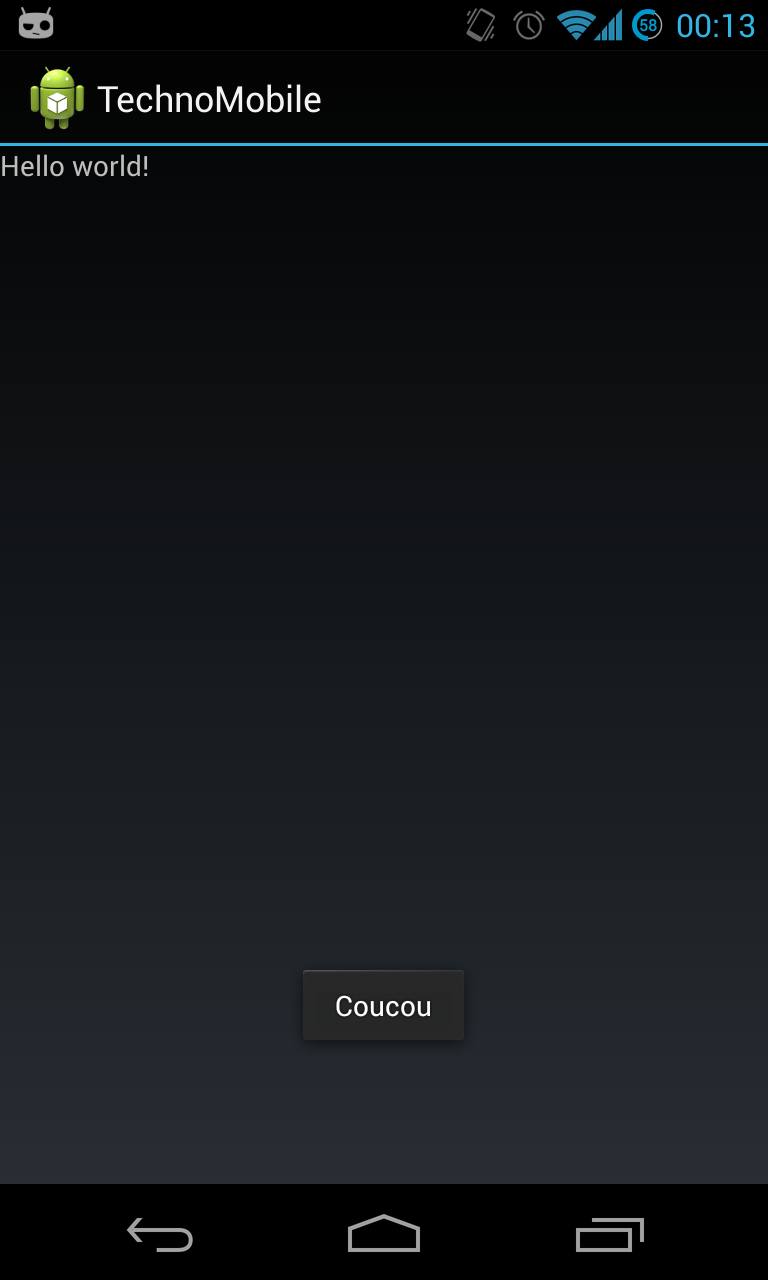
\includegraphics[width=60pt]{coucou.png}
\begin{lstlisting}
public MyActivity extends Activity {
    
    public void faireCoucou() {
        Toast.makeText(this,"Coucou",Toast.LENGTH_LONG).show();
        Toast.makeText(this,R.string.coucou,Toast.LENGTH_SHORT).show();
    }	
}
\end{lstlisting}
\end{frame}

\begin{frame}[fragile]
\frametitle{Les autres composants d'une application : les services}
\begin{itemize}
 \item Tâche en arrière plan (attention, pas automatiquement dans un thread séparé)
 \item Cycle de vie différent de celui d'une activity
 \item Pas d'interface graphique (sauf si une activity interroge le service)
 \item Exemples : lecteur MP3, client torrent, système de mise à jour, taskkiller \ldots
 \end{itemize}
\end{frame}
\begin{frame}[fragile]
\frametitle{Les autres composants d'une application : les broadcast receivers}
\begin{itemize}
 \item Composant recevant les annonces système et les annonces des autres applications
 \item Permet de réagir à certains évenements
 \item Possibilité de lancer des activités ou des services depuis le broadcast receiver
 \item Exemples : indicateur de batterie, antivirus, lancement au démarrage \ldots
 \end{itemize}
\end{frame}
\begin{frame}[fragile]
\frametitle{Les autres composants d'une application : les content-providers}
\begin{itemize}
  \item Composant servant à distribuer les données
  \item Peu importe comment les données sont stockées (sqlite, préferences, fichier \ldots)
  \item Respecte une interface d'utilisation des données
  \item Peut permettre la récupération, la modification et/ou la suppression de données
  \item Principalement déstiné à une utilisation entre applications
  \item Gestion de la sécurité et des droits (permissions)
  \item Exemple : accès au données système (SMS, contacts \ldots) 
 \end{itemize}
\end{frame}

\begin{frame}[fragile]
\frametitle{Les intents}
\begin{itemize}
 \item On déclare son intention, android réagit en conséquence
 \item Intents implicites ``Je veux ouvrir la page web \url{https://twitter.com/Ensai35}''
 \item ``Je veux envoyer un mail à jlegouic@ensai.fr avec le titre URGENT : FOOT''
 \item Intents explicites ``Je veux lancer l'activity MyActivity''
 \end{itemize}
\end{frame}
\begin{frame}[fragile]
\frametitle{Lancer un intent implicite}
\begin{lstlisting}
public MyActivity extends Activity {
    
    public void envoyerMail() {
        Intent i = new Intent(Intent.ACTION_SEND);
        i.setType("message/rfc822");
        i.putExtra(Intent.EXTRA_EMAIL  , "annee2@ensai.fr");
        i.putExtra(Intent.EXTRA_SUBJECT,"URGENT : FOOT"); 
        i.putExtra(Intent.EXTRA_TEXT   , "...");
        try {
            startActivity(i);
        } 
        catch (ActivityNotFoundException ex) {
            //Pas de client mail installe
        }
    }	
}
\end{lstlisting}
\end{frame}
\begin{frame}[fragile]
\frametitle{Lancer un intent explicite}
\begin{lstlisting}
public MyActivity extends Activity {
    
    public void lancerMyActivity2() {
        Intent intent = new Intent(this, MyActivity2.class); 
        //this fait reference a un context
        startActivity(intent);
    }	
}
\end{lstlisting}
\end{frame}

\begin{frame}[fragile]
\frametitle{Filtrer les intents, le principe}
\begin{itemize}
    \item startActivity(), startService() et sendBroadcast() déclenchent des
    intents
	\item android filtre les composants succeptibles de recevoir l'intent en
	fonction à partir des intent-filters de chaque composant
\end{itemize}

\begin{lstlisting}
<activity android:name="com.ensai.technomobile.MainActivity"
            android:label="@string/app_name" >
            <intent-filter>
                <action android:name="android.intent.action.MAIN" />
                <category android:name="android.intent.category.LAUNCHER" />
            </intent-filter>
        </activity>
\end{lstlisting}
\end{frame}
\begin{frame}[fragile]
\frametitle{Filtrer les intents, exemple}
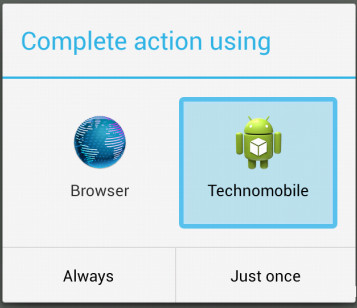
\includegraphics[width=45pt]{intentchooser.jpg}
\begin{lstlisting}
<activity
            android:name="com.ensai.technomobile.TwitterActivity"
            android:label="@string/app_name" >
            <intent-filter>
                <data
                    android:host="twitter.com"
                    android:scheme="http" />
                <category android:name="android.intent.category.DEFAULT" />
                <category android:name="android.intent.category.BROWSABLE" />
                <action android:name="android.intent.action.VIEW" />
            </intent-filter>
        </activity>
\end{lstlisting}
\end{frame}

\subsection{Les données}
\frametitle{Gestion des données}
\begin{frame}
Il existe plusieurs façons de stocker les données sur un appareil android
\begin{itemize}
    \item \textbf{SharedPreferences}: stockage de données primitives
    \item \textbf{Fichiers}: contenus sur la mémoire interne ou externe
    \item \textbf{Bases de données}: SQLite
    \item \textbf{Stockage distant}: webservice
\end{itemize}
Documentation android officielle sur le stockage de données : \url{http://developer.android.com/guide/topics/data/data-storage.html}
\end{frame}

\begin{frame}
\frametitle{SharedPreferences}
\begin{itemize}
    \item Equivalent des Preferences de java
    \item Stockage de données primitives (int, boolean, String \ldots)
    \item Mapping clé / valeur
    \item Très facile de créer un écran de paramètres (PreferenceActivity)
    \item Système de listeners pour être prévenu lors d'un changement
    \item Léger à implémenter
\end{itemize}
\end{frame}
\begin{frame}[fragile]
\frametitle{SharedPreferences, accéder aux préférences}
Accéder simple aux préferences :\\
\begin{lstlisting}
public void sauvegarderScore() {
    SharedPreferences preferences = PreferenceManager.getDefaultPreferences(context);
}
\end{lstlisting}
Accéder en précisant le nom et le mode :\\
\begin{lstlisting}
public void sauvegarderScore() {
    SharedPreferences preferences = context.getSharedPreferences("toto",Context.MODE_PRIVATE);
}
\end{lstlisting}
L'utilisation d'autres modes que MODE\_PRIVATE est découragé depuis l'API 17 (4.2) pour des raisons de sécurité.\\
\end{frame}
\begin{frame}[fragile]
\frametitle{SharedPreferences, utilisation des préférences}
Lire les préferences :\\
\begin{lstlisting}
public void afficherMeilleurScore() {
    SharedPreferences preferences = PreferenceManager.getDefaultPreferences(context);
    int record = preferences.getInt("meilleurScore");
    Toast.makeText(context, "Record : "+record,Toast.LENGTH_LONG).show();
}
\end{lstlisting}
Modifier les préferences\\
\begin{lstlisting}
public void sauvegarderScore() {
    SharedPreferences preferences = PreferenceManager.getDefaultPreferences(context);
    Editor editor = preferences.edit();
    editor.putInt("meilleurScore");
    editor.commit();
}
\end{lstlisting}
\end{frame}
\begin{frame}[fragile]
\frametitle{Les fichiers}
\begin{itemize}
    \item API classiques de java
    \item Ne jamais utiliser de chemin absolu, utiliser les fonctions android pour déterminer les dossiers
    \item Garder en tête les contraintes de place libre
    \item Choisir entre stockage interne et externe
\end{itemize}
\end{frame}
\begin{frame}[fragile]
\frametitle{Stockage interne}
\begin{lstlisting}
FileOutputStream fos = context.openFileOutput("monFichier.ext", Context.MODE_PRIVATE);
fos.write("texte".getBytes());
fos.close();
\end{lstlisting}
\begin{itemize}
    \item Comme pour les préférences, ne pas utiliser les modes WORLD\_READABLE et WORLD\_WRITEABLE
    \item MODE\_APPEND est utilisable pour écrire à la fin du fichier
    \item Les fichiers crées sur le stockage interne sont liés à l'application (en particulier, ils sont supprimés lors de la désinstallation de l'application)
\end{itemize}
\begin{itemize}
    \item getCacheDir() : répertoire pour le cache
    \item getFilesDir() : dossier où sont stockés les fichiers de l'application
    \item deleteFile(String nom)
    \item fileList() : String[] des fichiers crées par l'application
\end{itemize}
\end{frame}
\begin{frame}[fragile]
\frametitle{Stockage externe}
\begin{itemize}
    \item Far-west : l'utilisateur et toutes les applications peuvent lire / écrire tout le contenu
    \item La présence d'un stockage externe n'est pas garanti
    \item Même si il est présent, le stockage externe peut ne pas être disponible
\end{itemize}
\begin{lstlisting}
String state = Environment.getExternalStorageState();
if (Environment.MEDIA_MOUNTED.equals(state)) {
    //Lecture et ecriture possibles
} 
else if (Environment.MEDIA_MOUNTED_READ_ONLY.equals(state)) {
    //Ecriture impossible, lecture possible
} 
else {
    //Lecture et ecriture impossibles
}
\end{lstlisting}
\end{frame}
\begin{frame}[fragile]
\frametitle{Stockage externe, utilisation}
Pour le contenu utilisé uniquement par l'application :
\begin{lstlisting}
File file = new File(getExternalFilesDir(null), "DemoFile.jpg");
\end{lstlisting}
Ces fichiers seront supprimés lors de la désinstallation de l'application\\\\
Pour le contenu déstiné à être partagé (donc persistant même après une désinstallation) : 
\begin{lstlisting}
File file = new File(getExternalStoragePublicDirectory(Environment.DIRECTORY_PICTURES), "DemoFile.jpg");
\end{lstlisting}
L'argument utilisé dans les 2 cas correspond au type de données et est une variable static de Environment\\
Exemples : Environment.DIRECTORY\_PICTURES, DIRECTORY\_MUSIC, DIRECTORY\_DOWNLOADS, DIRECTORY\_DCIM \ldots
\end{frame}
\begin{frame}[fragile]
\frametitle{SQLite, le moteur de base de données embarqué}
\begin{itemize}
    \item SQLite est un moteur de base de données spécialement conçu pour le mobie et l'embarqué
    \item On retrouve à peu près l'ensemble des fonctions de base d'un moteur de BDD
    \item Android propose en plus une API facilitant les tâches courantes : SQLiteOpenHelper
    \item Pour les requêtes, android offre une API proche de JDBC
\end{itemize}
\end{frame}
\begin{frame}[fragile]
\frametitle{Mise en place d'une base de données SQLite}
Etape 1 : étendre SQLiteOpenHelper 
\begin{lstlisting}
public class MyOpenHelper extends SQLiteOpenHelper {

    private static final int DATABASE_VERSION = 1;
    private static final String DATABASE_NAME = "mabase";

    public MyOpenHelper(Context context) {
        super(context, DATABASE_NAME, null, DATABASE_VERSION);
    }
}
\end{lstlisting}
Etape 2 : implémenter onCreate
\begin{lstlisting}
    @Override
    public void onCreate(SQLiteDatabase db) {
        db.execSQL("CREATE TABLE exemple (nom TEXT PRIMARY KEY, score INTEGER));
    }
\end{lstlisting}
\end{frame}
\begin{frame}[fragile]
\frametitle{Mise en place d'une base de données SQLite}
Etape 3 : Organiser les mises à jour de la base
\begin{lstlisting}
public class MyOpenHelper extends SQLiteOpenHelper {
    @Override
    public void onUpgrade(SQLiteDatabase db, int oldVersion, int newVersion) {
        //Mise a jour de la base si besoin
    }
}
\end{lstlisting}
\begin{itemize}
    \item L'entier DATABASE\_VERSION permet de savoir si une mise à jour de la base est nécessaire
    \item Android appelle directement onUpgrade si le numéro de version est supérieur au numéro de version actuel de la base
    \item onUpgrade doît alors faire les mises à jour qui s'impose en fonction des entiers oldVersion / newVersion 
\end{itemize}
\end{frame}
\begin{frame}[fragile]
\frametitle{Utilisation de SQLite}
Récupérer une instance de SQLiteDatabase
\begin{lstlisting}
SQLiteOpenHelper helper = new SQLiteOpenHelper(context);
SQLiteDatabase writableDB = helper.getWritableDatabase();
SQLiteDatabase readableDB = helper.getReadableDatabase();
\end{lstlisting}
\begin{itemize}
    \item Android propose un certain nombre de fonctions utilitaires pour le requêtage, l'insertion, la mise à jour et la suppresion de données
    \item Penser à fermer la base avec .close() pour libérer des ressources
\end{itemize}
\end{frame}
\begin{frame}[fragile]
\frametitle{Utilisation de SQLite, les requêtes}
\begin{itemize}
    \item 2 méthodes au choix en fonction du besoin
    \item Ces méthodes sont déclinées en de multiples méthodes (surcharge)
    \item rawQuery(String sql, String[] selectionArgs) pour du sql dur ({\raise.17ex\hbox{$\scriptstyle\sim$}} PreparedStatement)
    \item query(String table, String[] columns, String selection, String[] selectionArgs, String groupBy, String having, String orderBy) pour que android génère le sql
\end{itemize}
\begin{lstlisting}
SQLiteDatabase writableDB = helper.getWritableDatabase();
Cursor cursor1 = writableDB.rawQuery("SELECT nom,score FROM table WHERE id = ?",new String[] {"42"});
Cursor cursor2 = writableDB.query("table",new String[] {"nom","score"}, "id = ?",new String[] {"42"}, null, null, null );
\end{lstlisting}
\end{frame}
\begin{frame}[fragile]
\frametitle{Utilisation de SQLite, les cursors}
\begin{itemize}
    \item Wrappers autour d'un ResultSet
    \item Utilisation très proche des resultSets
    \item Penser à le fermer (close()) pour libérer des ressources
\end{itemize}
\begin{lstlisting}
int nbRows = cursor.getCount();
while (cursor.moveToNext()) {
    String nom = cursor.getString(0);
    int score = cursor.getInt(1);
}
cursor.close();
\end{lstlisting}
\end{frame}
\begin{frame}[fragile]
\frametitle{Utilisation de SQLite : update, insert et delete}
long insert (String table, String nullColumnHack, ContentValues values)
\begin{lstlisting}
ContentValues values = new ContentValues();
values.put("nom", "bob");
values.put("score", 42);
long rowID = bdd.insert(table, null, values);
\end{lstlisting}
int update(String table, ContentValues values, String whereClause, String[] whereArgs)
\begin{lstlisting}
ContentValues values = new ContentValues();
values.put("score", 42);
int nbRowsAffected = bdd.update(table, values, "nom = ?",new String[] {"42"});
\end{lstlisting}
int delete (String table, String whereClause, String[] whereArgs)
\begin{lstlisting}
int nbRowsAffected = bdd.delete(table,"nom = ?", new String[] {"bobette});
\end{lstlisting}
\end{frame}
\end{document}
